\section{Risk Triage: Robust Boundary, Weak Generalization}
The risk-aware layer is subordinate to the ACL and should be evaluated separately from the structural authorization guarantee. On the primary authorized-but-suspicious set, the fuzzy controller challenges or denies 88.0\% of requests, while the deterministic-rule comparator challenges 100\%. On the lexically disjoint held-out suspicious set, those rates collapse to 16.7\% and 16.0\%, respectively (Fig.~\ref{fig:risk}). Neither controller denies a held-out authorized-suspicious request; most are indistinguishable from benign prompts under the frozen lexical features.

\begin{figure}[t]
\centering
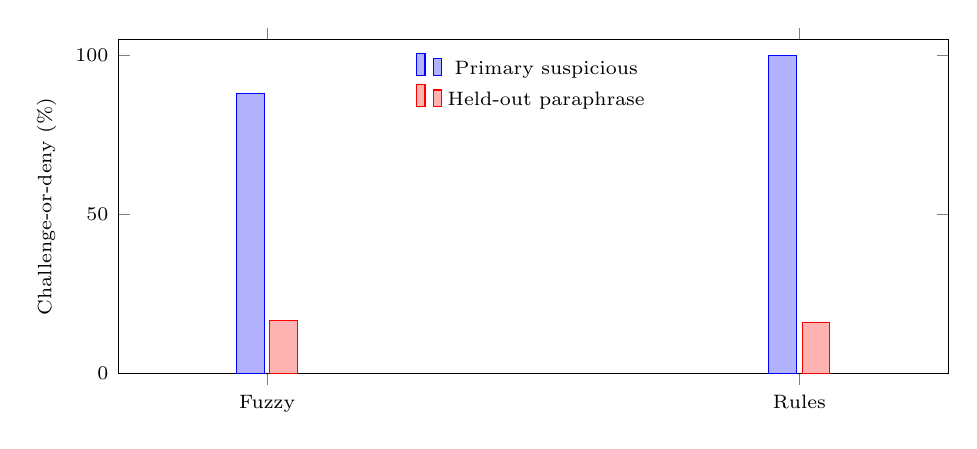
\begin{tikzpicture}
\begin{axis}[
  width=\columnwidth,height=0.48\columnwidth,
  ybar,bar width=10pt,ymin=0,ymax=105,
  ylabel={Challenge-or-deny (\%)},
  symbolic x coords={Fuzzy,Rules},xtick=data,
  xticklabel style={font=\scriptsize},
  yticklabel style={font=\scriptsize},
  label style={font=\scriptsize},
  legend style={font=\scriptsize,draw=none,at={(0.5,0.98)},anchor=north,legend columns=1},
  enlarge x limits=0.28]
\addplot coordinates {(Fuzzy,88.0) (Rules,100.0)};
\addplot coordinates {(Fuzzy,16.7) (Rules,16.0)};
\legend{Primary suspicious,Held-out paraphrase}
\end{axis}
\end{tikzpicture}
\caption{Suspicion-triage generalization. Structural unauthorized-target denial remains 100\% for both controllers, but suspicious-authorized challenge rates collapse under held-out paraphrases.}
\label{fig:risk}
\end{figure}

By contrast, unauthorized-target denial is 100\% for both controllers on both primary and held-out sets. This is not evidence that the heuristic detector generalizes; it follows from authorization confidence and the ACL boundary. The fuzzy-vs-rule paired challenge comparison over the combined evaluation yields $p=0.0043$, but the direction is not a fuzzy advantage: deterministic rules challenge more in-distribution cases and the two are nearly identical out of distribution. We therefore present fuzzy logic only as one adaptive policy mechanism and make no claim that it outperforms transparent threshold rules.

\begin{table}[t]
\caption{Risk-triage behavior on authorized-suspicious requests.}
\label{tab:risk}
\centering
\footnotesize
\begin{tabular}{lrr}
\toprule
Controller & Primary & Held-out paraphrase \\
\midrule
Fuzzy challenge-or-deny & 88.0\% & 16.7\% \\
Deterministic rules & 100.0\% & 16.0\% \\
Fuzzy deny only & 26.4\% & 0.0\% \\
Rules deny only & 50.4\% & 0.0\% \\
\bottomrule
\end{tabular}
\end{table}

The alias-free benchmark further tests a separate robustness question. Queries identify a synthetic patient by name rather than by \texttt{PAT-xxxx} alias. Authorized target resolution succeeds in 100/100 cases for both secured architectures; unauthorized target resolution/retrieval is 0/100, because candidate filtering remains limited to authorized aliases even when direct alias parsing is absent. This supports a bounded claim about name-based resolution in the implemented retriever, not general identifier robustness.
